\documentclass[twoside]{book}

% Packages required by doxygen
\usepackage{calc}
\usepackage{doxygen}
\usepackage{graphicx}
\usepackage[utf8]{inputenc}
\usepackage{makeidx}
\usepackage{multicol}
\usepackage{multirow}
\usepackage{textcomp}
\usepackage[table]{xcolor}

% Font selection
\usepackage[T1]{fontenc}
\usepackage{mathptmx}
\usepackage[scaled=.90]{helvet}
\usepackage{courier}
\usepackage{amssymb}
\usepackage{sectsty}
\renewcommand{\familydefault}{\sfdefault}
\allsectionsfont{%
  \fontseries{bc}\selectfont%
  \color{darkgray}%
}
\renewcommand{\DoxyLabelFont}{%
  \fontseries{bc}\selectfont%
  \color{darkgray}%
}

% Page & text layout
\usepackage{geometry}
\geometry{%
  a4paper,%
  top=2.5cm,%
  bottom=2.5cm,%
  left=2.5cm,%
  right=2.5cm%
}
\tolerance=750
\hfuzz=15pt
\hbadness=750
\setlength{\emergencystretch}{15pt}
\setlength{\parindent}{0cm}
\setlength{\parskip}{0.2cm}
\makeatletter
\renewcommand{\paragraph}{%
  \@startsection{paragraph}{4}{0ex}{-1.0ex}{1.0ex}{%
    \normalfont\normalsize\bfseries\SS@parafont%
  }%
}
\renewcommand{\subparagraph}{%
  \@startsection{subparagraph}{5}{0ex}{-1.0ex}{1.0ex}{%
    \normalfont\normalsize\bfseries\SS@subparafont%
  }%
}
\makeatother

% Headers & footers
\usepackage{fancyhdr}
\pagestyle{fancyplain}
\fancyhead[LE]{\fancyplain{}{\bfseries\thepage}}
\fancyhead[CE]{\fancyplain{}{}}
\fancyhead[RE]{\fancyplain{}{\bfseries\leftmark}}
\fancyhead[LO]{\fancyplain{}{\bfseries\rightmark}}
\fancyhead[CO]{\fancyplain{}{}}
\fancyhead[RO]{\fancyplain{}{\bfseries\thepage}}
\fancyfoot[LE]{\fancyplain{}{}}
\fancyfoot[CE]{\fancyplain{}{}}
\fancyfoot[RE]{\fancyplain{}{\bfseries\scriptsize Generated on Wed Jun 26 2013 00:31:28 for Sudoku by Doxygen }}
\fancyfoot[LO]{\fancyplain{}{\bfseries\scriptsize Generated on Wed Jun 26 2013 00:31:28 for Sudoku by Doxygen }}
\fancyfoot[CO]{\fancyplain{}{}}
\fancyfoot[RO]{\fancyplain{}{}}
\renewcommand{\footrulewidth}{0.4pt}
\renewcommand{\chaptermark}[1]{%
  \markboth{#1}{}%
}
\renewcommand{\sectionmark}[1]{%
  \markright{\thesection\ #1}%
}

% Indices & bibliography
\usepackage{natbib}
\usepackage[titles]{tocloft}
\setcounter{tocdepth}{3}
\setcounter{secnumdepth}{5}
\makeindex

% Hyperlinks (required, but should be loaded last)
\usepackage{ifpdf}
\ifpdf
  \usepackage[pdftex,pagebackref=true]{hyperref}
\else
  \usepackage[ps2pdf,pagebackref=true]{hyperref}
\fi
\hypersetup{%
  colorlinks=true,%
  linkcolor=blue,%
  citecolor=blue,%
  unicode%
}

% Custom commands
\newcommand{\clearemptydoublepage}{%
  \newpage{\pagestyle{empty}\cleardoublepage}%
}


%===== C O N T E N T S =====

\begin{document}

% Titlepage & ToC
\hypersetup{pageanchor=false}
\pagenumbering{roman}
\begin{titlepage}
\vspace*{7cm}
\begin{center}%
{\Large Sudoku \\[1ex]\large 1.\-0 }\\
\vspace*{1cm}
{\large Generated by Doxygen 1.8.4}\\
\vspace*{0.5cm}
{\small Wed Jun 26 2013 00:31:28}\\
\end{center}
\end{titlepage}
\clearemptydoublepage
\tableofcontents
\clearemptydoublepage
\pagenumbering{arabic}
\hypersetup{pageanchor=true}

%--- Begin generated contents ---
\chapter{Hierarchical Index}
\section{Class Hierarchy}
This inheritance list is sorted roughly, but not completely, alphabetically\-:\begin{DoxyCompactList}
\item \contentsline{section}{Dimensiones}{\pageref{class_dimensiones}}{}
\item \contentsline{section}{Generador}{\pageref{class_generador}}{}
\item Q\-Main\-Window\begin{DoxyCompactList}
\item \contentsline{section}{Main\-Window}{\pageref{class_main_window}}{}
\end{DoxyCompactList}
\item Q\-Widget\begin{DoxyCompactList}
\item \contentsline{section}{Numero}{\pageref{class_numero}}{}
\end{DoxyCompactList}
\end{DoxyCompactList}

\chapter{Class Index}
\section{Class List}
Here are the classes, structs, unions and interfaces with brief descriptions\-:\begin{DoxyCompactList}
\item\contentsline{section}{\hyperlink{class_dimensiones}{Dimensiones} }{\pageref{class_dimensiones}}{}
\item\contentsline{section}{\hyperlink{class_generador}{Generador} }{\pageref{class_generador}}{}
\item\contentsline{section}{\hyperlink{class_main_window}{Main\-Window} }{\pageref{class_main_window}}{}
\item\contentsline{section}{\hyperlink{class_numero}{Numero} }{\pageref{class_numero}}{}
\end{DoxyCompactList}

\chapter{File Index}
\section{File List}
Here is a list of all documented files with brief descriptions\-:\begin{DoxyCompactList}
\item\contentsline{section}{C\-:/\-Users/user/\-Documents/\-Git\-Hub/\-Sudoku/\-Sudoku/{\bfseries Dimensiones.\-h} }{\pageref{_dimensiones_8h}}{}
\item\contentsline{section}{C\-:/\-Users/user/\-Documents/\-Git\-Hub/\-Sudoku/\-Sudoku/\hyperlink{generador_8h}{generador.\-h} \\*Este archivo contiene la interfaz del generador de Sudokus }{\pageref{generador_8h}}{}
\item\contentsline{section}{C\-:/\-Users/user/\-Documents/\-Git\-Hub/\-Sudoku/\-Sudoku/\hyperlink{mainwindow_8h}{mainwindow.\-h} \\*Este archivo contiene la interfaz de la ventana principal }{\pageref{mainwindow_8h}}{}
\item\contentsline{section}{C\-:/\-Users/user/\-Documents/\-Git\-Hub/\-Sudoku/\-Sudoku/{\bfseries Mejores\-Puntajes.\-h} }{\pageref{_mejores_puntajes_8h}}{}
\item\contentsline{section}{C\-:/\-Users/user/\-Documents/\-Git\-Hub/\-Sudoku/\-Sudoku/{\bfseries mejorestiempos.\-h} }{\pageref{mejorestiempos_8h}}{}
\item\contentsline{section}{C\-:/\-Users/user/\-Documents/\-Git\-Hub/\-Sudoku/\-Sudoku/\hyperlink{numero_8h}{numero.\-h} \\*Este archivo contiene la interfaz de la clase \hyperlink{class_numero}{Numero} }{\pageref{numero_8h}}{}
\item\contentsline{section}{C\-:/\-Users/user/\-Documents/\-Git\-Hub/\-Sudoku/\-Sudoku/\hyperlink{_posicion_8h}{Posicion.\-h} \\*Este archivo contiene la interfaz de la clase \hyperlink{class_posicion}{Posicion} }{\pageref{_posicion_8h}}{}
\item\contentsline{section}{C\-:/\-Users/user/\-Documents/\-Git\-Hub/\-Sudoku/\-Sudoku/\hyperlink{puntaje_8h}{puntaje.\-h} \\*Este archivo contiene la interfaz de la clase \hyperlink{class_puntaje}{Puntaje} }{\pageref{puntaje_8h}}{}
\end{DoxyCompactList}

\chapter{Class Documentation}
\hypertarget{class_dimensiones}{\section{Dimensiones Class Reference}
\label{class_dimensiones}\index{Dimensiones@{Dimensiones}}
}
\subsection*{Static Public Attributes}
\begin{DoxyCompactItemize}
\item 
\hypertarget{class_dimensiones_a2fb9391d1230b6cc7a2a4008e74bcddc}{static const int {\bfseries margin} = 10}\label{class_dimensiones_a2fb9391d1230b6cc7a2a4008e74bcddc}

\item 
\hypertarget{class_dimensiones_a961ddc06835eac206208ca5069d935b7}{static const int {\bfseries numero\-Size} = 50}\label{class_dimensiones_a961ddc06835eac206208ca5069d935b7}

\item 
\hypertarget{class_dimensiones_ade4db223d06ae4688d1f39835bdb4654}{static const int {\bfseries tablero\-Size} = numero\-Size $\ast$ 9 + 4 $\ast$ margin}\label{class_dimensiones_ade4db223d06ae4688d1f39835bdb4654}

\end{DoxyCompactItemize}


The documentation for this class was generated from the following file\-:\begin{DoxyCompactItemize}
\item 
C\-:/\-Users/user/\-Documents/\-Git\-Hub/\-Sudoku/\-Sudoku/Dimensiones.\-h\end{DoxyCompactItemize}

\hypertarget{class_generador}{\section{Generador Class Reference}
\label{class_generador}\index{Generador@{Generador}}
}
\subsection*{Public Member Functions}
\begin{DoxyCompactItemize}
\item 
\hypertarget{class_generador_ab67862d2f13c1e9b18b29b385bf5a20e}{void {\bfseries Generar\-Tablero} (int dificultad)}\label{class_generador_ab67862d2f13c1e9b18b29b385bf5a20e}

\item 
\hypertarget{class_generador_a430dccdbfe57088212912c30259f8757}{bool {\bfseries resolver\-Tablero} ()}\label{class_generador_a430dccdbfe57088212912c30259f8757}

\item 
\hypertarget{class_generador_a0e8bb058054de56ece51fc880a23fd07}{bool {\bfseries escanear\-Solucion} ()}\label{class_generador_a0e8bb058054de56ece51fc880a23fd07}

\end{DoxyCompactItemize}
\subsection*{Public Attributes}
\begin{DoxyCompactItemize}
\item 
\hypertarget{class_generador_ab990ce2cbce0dcf52b0ed827545e0b16}{int $\ast$ {\bfseries tablero}}\label{class_generador_ab990ce2cbce0dcf52b0ed827545e0b16}

\end{DoxyCompactItemize}


The documentation for this class was generated from the following files\-:\begin{DoxyCompactItemize}
\item 
Sudoku/generador.\-h\item 
Sudoku/generador.\-cpp\end{DoxyCompactItemize}

\hypertarget{class_main_window}{\section{Main\-Window Class Reference}
\label{class_main_window}\index{Main\-Window@{Main\-Window}}
}
Inheritance diagram for Main\-Window\-:\begin{figure}[H]
\begin{center}
\leavevmode
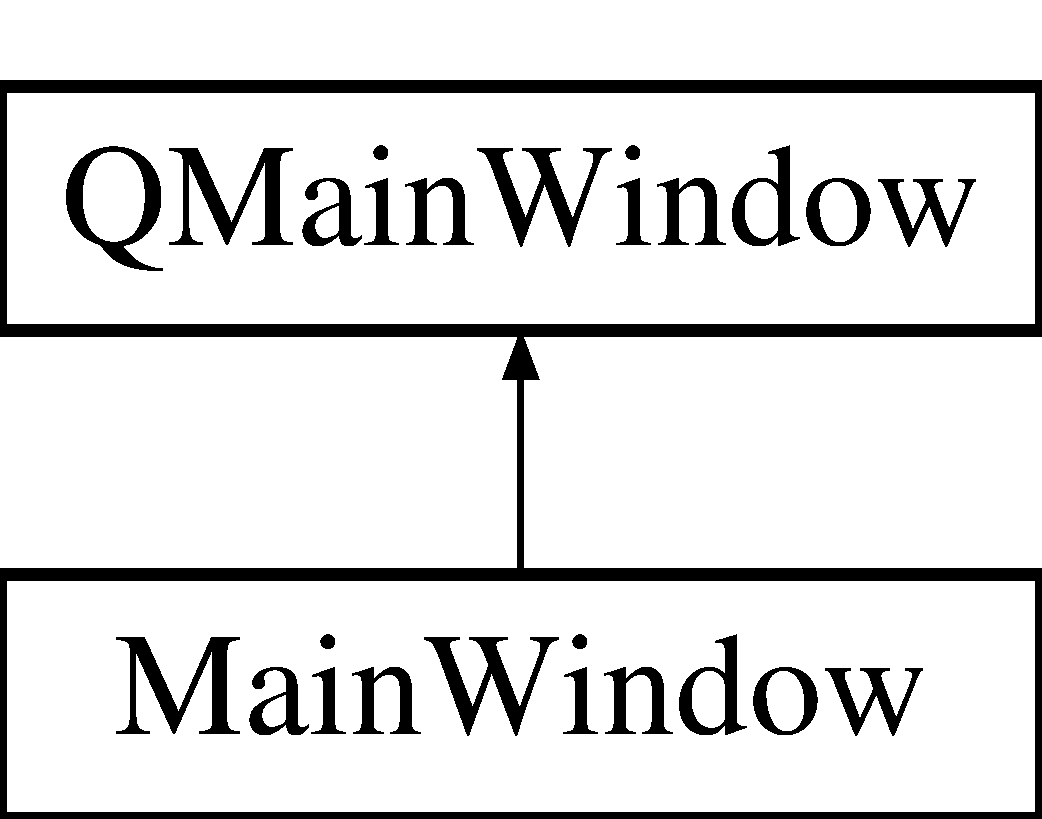
\includegraphics[height=2.000000cm]{class_main_window}
\end{center}
\end{figure}
\subsection*{Public Member Functions}
\begin{DoxyCompactItemize}
\item 
\hyperlink{class_main_window_a8b244be8b7b7db1b08de2a2acb9409db}{Main\-Window} (Q\-Widget $\ast$parent=0)
\item 
bool \hyperlink{class_main_window_adb7dbe0ece2eaa1a92b3ee1da8ae3327}{jugada\-Valida} (int casilla, int valor)
\item 
bool \hyperlink{class_main_window_ab68ff992b159d33b1f80606deabe0361}{jugada\-Correcta} (int casilla)
\item 
void \hyperlink{class_main_window_a18e451ac33947c4e8c058a5266daafbd}{creacion\-Numeros} (int indice, int valor\-Correcto, int col, int fila, int visible)
\item 
void \hyperlink{class_main_window_af0799066013e5dac6614367dc715d3e4}{creacion\-Botones} ()
\item 
void \hyperlink{class_main_window_ade1681f57a1c4cacefd88030c3f70b23}{inicializar\-Timer} ()
\item 
\hyperlink{class_main_window_ae98d00a93bc118200eeef9f9bba1dba7}{$\sim$\-Main\-Window} ()
\end{DoxyCompactItemize}


\subsection{Constructor \& Destructor Documentation}
\hypertarget{class_main_window_a8b244be8b7b7db1b08de2a2acb9409db}{\index{Main\-Window@{Main\-Window}!Main\-Window@{Main\-Window}}
\index{Main\-Window@{Main\-Window}!MainWindow@{Main\-Window}}
\subsubsection[{Main\-Window}]{\setlength{\rightskip}{0pt plus 5cm}Main\-Window\-::\-Main\-Window (
\begin{DoxyParamCaption}
\item[{Q\-Widget $\ast$}]{parent = {\ttfamily 0}}
\end{DoxyParamCaption}
)\hspace{0.3cm}{\ttfamily [explicit]}}}\label{class_main_window_a8b244be8b7b7db1b08de2a2acb9409db}
\hyperlink{class_main_window}{Main\-Window} Constructor de la clase \hyperlink{class_main_window}{Main\-Window} 
\begin{DoxyParams}{Parameters}
{\em parent} & Padre de la clase \\
\hline
\end{DoxyParams}
\hypertarget{class_main_window_ae98d00a93bc118200eeef9f9bba1dba7}{\index{Main\-Window@{Main\-Window}!$\sim$\-Main\-Window@{$\sim$\-Main\-Window}}
\index{$\sim$\-Main\-Window@{$\sim$\-Main\-Window}!MainWindow@{Main\-Window}}
\subsubsection[{$\sim$\-Main\-Window}]{\setlength{\rightskip}{0pt plus 5cm}Main\-Window\-::$\sim$\-Main\-Window (
\begin{DoxyParamCaption}
{}
\end{DoxyParamCaption}
)}}\label{class_main_window_ae98d00a93bc118200eeef9f9bba1dba7}
$\sim$\-Main\-Window Destructor de la clase \hyperlink{class_main_window}{Main\-Window} 

\subsection{Member Function Documentation}
\hypertarget{class_main_window_af0799066013e5dac6614367dc715d3e4}{\index{Main\-Window@{Main\-Window}!creacion\-Botones@{creacion\-Botones}}
\index{creacion\-Botones@{creacion\-Botones}!MainWindow@{Main\-Window}}
\subsubsection[{creacion\-Botones}]{\setlength{\rightskip}{0pt plus 5cm}void Main\-Window\-::creacion\-Botones (
\begin{DoxyParamCaption}
{}
\end{DoxyParamCaption}
)}}\label{class_main_window_af0799066013e5dac6614367dc715d3e4}
creacion\-Botones Crea un tablero de numeros. \hypertarget{class_main_window_a18e451ac33947c4e8c058a5266daafbd}{\index{Main\-Window@{Main\-Window}!creacion\-Numeros@{creacion\-Numeros}}
\index{creacion\-Numeros@{creacion\-Numeros}!MainWindow@{Main\-Window}}
\subsubsection[{creacion\-Numeros}]{\setlength{\rightskip}{0pt plus 5cm}void Main\-Window\-::creacion\-Numeros (
\begin{DoxyParamCaption}
\item[{int}]{indice, }
\item[{int}]{valor\-Correcto, }
\item[{int}]{col, }
\item[{int}]{fila, }
\item[{int}]{visible}
\end{DoxyParamCaption}
)}}\label{class_main_window_a18e451ac33947c4e8c058a5266daafbd}
creacion\-Numeros Crea un numero y lo agrega al tablero. 
\begin{DoxyParams}{Parameters}
{\em indice} & Indice del arreglo numeros que determina la casilla. \\
\hline
{\em valor\-Correcto} & Valor que se asigna en la generacion del tablero. \\
\hline
{\em col} & Columna a la que corresponde el numero. \\
\hline
{\em fila} & Fila a la que corresponde el numero. \\
\hline
{\em visible} & Verdadero si el numero debe mostrarse, falso si la casilla debe mostrarse vacia. \\
\hline
\end{DoxyParams}
\hypertarget{class_main_window_ade1681f57a1c4cacefd88030c3f70b23}{\index{Main\-Window@{Main\-Window}!inicializar\-Timer@{inicializar\-Timer}}
\index{inicializar\-Timer@{inicializar\-Timer}!MainWindow@{Main\-Window}}
\subsubsection[{inicializar\-Timer}]{\setlength{\rightskip}{0pt plus 5cm}void Main\-Window\-::inicializar\-Timer (
\begin{DoxyParamCaption}
{}
\end{DoxyParamCaption}
)}}\label{class_main_window_ade1681f57a1c4cacefd88030c3f70b23}
inicializar\-Timer Inicializa el cronometro. \hypertarget{class_main_window_ab68ff992b159d33b1f80606deabe0361}{\index{Main\-Window@{Main\-Window}!jugada\-Correcta@{jugada\-Correcta}}
\index{jugada\-Correcta@{jugada\-Correcta}!MainWindow@{Main\-Window}}
\subsubsection[{jugada\-Correcta}]{\setlength{\rightskip}{0pt plus 5cm}bool Main\-Window\-::jugada\-Correcta (
\begin{DoxyParamCaption}
\item[{int}]{casilla}
\end{DoxyParamCaption}
)}}\label{class_main_window_ab68ff992b159d33b1f80606deabe0361}
jugada\-Valida Determina si una jugada es correcta. 
\begin{DoxyParams}{Parameters}
{\em casilla} & Indice del arreglo numeros que determina la casilla. \\
\hline
{\em valor} & \hyperlink{class_numero}{Numero} que se esta asignando en la casilla \\
\hline
\end{DoxyParams}
\begin{DoxyReturn}{Returns}
Verdadero si la jugada es correcta, falso si no lo es. 
\end{DoxyReturn}
\hypertarget{class_main_window_adb7dbe0ece2eaa1a92b3ee1da8ae3327}{\index{Main\-Window@{Main\-Window}!jugada\-Valida@{jugada\-Valida}}
\index{jugada\-Valida@{jugada\-Valida}!MainWindow@{Main\-Window}}
\subsubsection[{jugada\-Valida}]{\setlength{\rightskip}{0pt plus 5cm}bool Main\-Window\-::jugada\-Valida (
\begin{DoxyParamCaption}
\item[{int}]{casilla, }
\item[{int}]{valor}
\end{DoxyParamCaption}
)}}\label{class_main_window_adb7dbe0ece2eaa1a92b3ee1da8ae3327}
jugada\-Valida Determina si una jugada es valida 
\begin{DoxyParams}{Parameters}
{\em casilla} & Indice del arreglo numeros que determina la casilla. \\
\hline
{\em valor} & \hyperlink{class_numero}{Numero} que se esta asignando en la casilla \\
\hline
\end{DoxyParams}
\begin{DoxyReturn}{Returns}
Verdadero si la jugada es valida, falso si no lo es. 
\end{DoxyReturn}


The documentation for this class was generated from the following files\-:\begin{DoxyCompactItemize}
\item 
Sudoku/\hyperlink{mainwindow_8h}{mainwindow.\-h}\item 
Sudoku/mainwindow.\-cpp\end{DoxyCompactItemize}

\hypertarget{class_numero}{\section{Numero Class Reference}
\label{class_numero}\index{Numero@{Numero}}
}
Inheritance diagram for Numero\-:\begin{figure}[H]
\begin{center}
\leavevmode
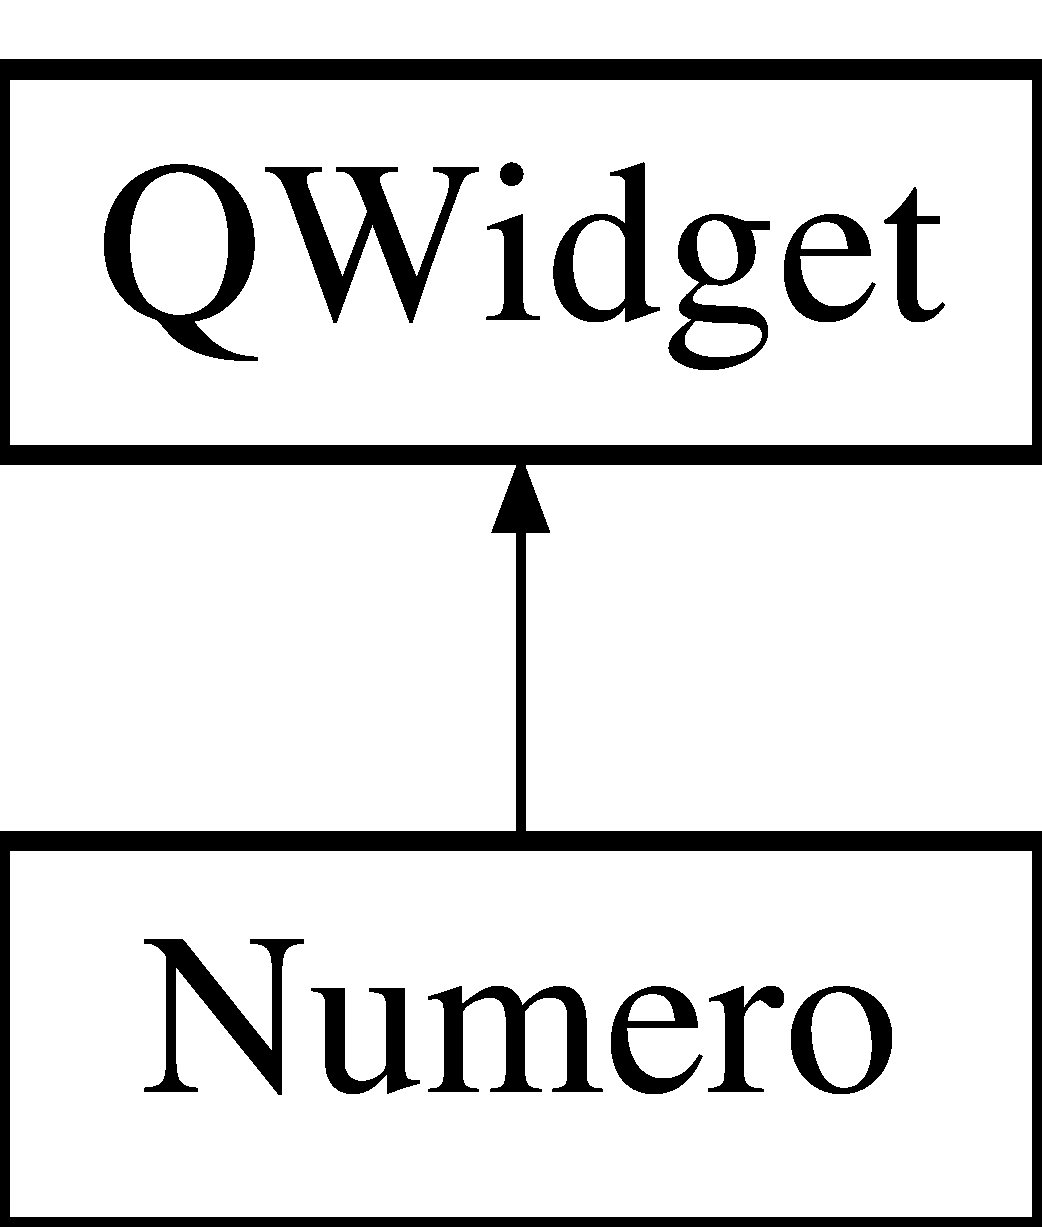
\includegraphics[height=2.000000cm]{class_numero}
\end{center}
\end{figure}
\subsection*{Public Member Functions}
\begin{DoxyCompactItemize}
\item 
\hypertarget{class_numero_a1393437877ace236d969c6dc44ae7ed4}{{\bfseries Numero} (Q\-Object $\ast$parent=0)}\label{class_numero_a1393437877ace236d969c6dc44ae7ed4}

\item 
\hypertarget{class_numero_a390143320c62c9ec5f89d767b8c2ef33}{{\bfseries Numero} (int numero, int columna, int fila, bool visible)}\label{class_numero_a390143320c62c9ec5f89d767b8c2ef33}

\item 
\hypertarget{class_numero_a582df3fe258d20235163d0fbcec712a8}{void {\bfseries set\-Cuadricula} (int fila, int columna)}\label{class_numero_a582df3fe258d20235163d0fbcec712a8}

\item 
\hypertarget{class_numero_a836200e8bd04882bc7ea2f5bc5d7beef}{void {\bfseries set\-Valor} (int valor)}\label{class_numero_a836200e8bd04882bc7ea2f5bc5d7beef}

\item 
\hypertarget{class_numero_ae9002d90ee6ccd3120077c304b85f4fd}{void {\bfseries set\-Valor\-Correcto} (int valor)}\label{class_numero_ae9002d90ee6ccd3120077c304b85f4fd}

\item 
\hypertarget{class_numero_a611e944da6a63813e305287c3f90ad76}{int {\bfseries get\-Fila} (void) const }\label{class_numero_a611e944da6a63813e305287c3f90ad76}

\item 
\hypertarget{class_numero_a4420f97d86be1c1a173405ea37423449}{int {\bfseries get\-Columna} (void) const }\label{class_numero_a4420f97d86be1c1a173405ea37423449}

\item 
\hypertarget{class_numero_ac80a32905356e20d893807572f8b8d4a}{int {\bfseries get\-Cuadricula} (void) const }\label{class_numero_ac80a32905356e20d893807572f8b8d4a}

\item 
\hypertarget{class_numero_ab744d258e626684a3106d39c9cf630b7}{int {\bfseries get\-Valor} (void) const }\label{class_numero_ab744d258e626684a3106d39c9cf630b7}

\item 
\hypertarget{class_numero_a850682763636579e94c90579f74d1308}{int {\bfseries get\-Valor\-Correcto} (void) const }\label{class_numero_a850682763636579e94c90579f74d1308}

\item 
\hypertarget{class_numero_a318e925fff822ed78cd39e382543620c}{void {\bfseries editar\-Boton} (int n)}\label{class_numero_a318e925fff822ed78cd39e382543620c}

\item 
\hypertarget{class_numero_a8a2040801509a6563189dac2a6618372}{void {\bfseries cambiar\-Color\-Boton\-Alerta} ()}\label{class_numero_a8a2040801509a6563189dac2a6618372}

\item 
\hypertarget{class_numero_a1492e35dd63ed7c2a0b6505f755fbf28}{void {\bfseries cambiar\-Color\-Boton\-Pista} ()}\label{class_numero_a1492e35dd63ed7c2a0b6505f755fbf28}

\item 
\hypertarget{class_numero_a8508989f8472de04dd6a4509d1e15814}{void {\bfseries cambiar\-Color\-Boton\-Original} ()}\label{class_numero_a8508989f8472de04dd6a4509d1e15814}

\end{DoxyCompactItemize}
\subsection*{Public Attributes}
\begin{DoxyCompactItemize}
\item 
\hypertarget{class_numero_ae868309035237d255665cc47e11f358e}{Q\-Label $\ast$ {\bfseries label\-Number}}\label{class_numero_ae868309035237d255665cc47e11f358e}

\item 
\hypertarget{class_numero_a05c25be5d0eec99f68ecee2d362a1006}{Q\-Line\-Edit $\ast$ {\bfseries text\-Opciones}}\label{class_numero_a05c25be5d0eec99f68ecee2d362a1006}

\item 
\hypertarget{class_numero_a72aae20a1d5d8722c9da4fa8e97d4efc}{Q\-Push\-Button $\ast$ {\bfseries boton}}\label{class_numero_a72aae20a1d5d8722c9da4fa8e97d4efc}

\item 
\hypertarget{class_numero_a47f3d0b00a7f0c276326be98accb8afa}{Q\-String $\ast$ {\bfseries numero}}\label{class_numero_a47f3d0b00a7f0c276326be98accb8afa}

\end{DoxyCompactItemize}


The documentation for this class was generated from the following files\-:\begin{DoxyCompactItemize}
\item 
Sudoku/\hyperlink{numero_8h}{numero.\-h}\item 
Sudoku/numero.\-cpp\end{DoxyCompactItemize}

\chapter{File Documentation}
\hypertarget{numero_8h}{\section{Sudoku/numero.h File Reference}
\label{numero_8h}\index{Sudoku/numero.\-h@{Sudoku/numero.\-h}}
}


Este archivo contiene la interfaz de la clase \hyperlink{class_numero}{Numero}.  


{\ttfamily \#include $<$Q\-Widget$>$}\\*
{\ttfamily \#include $<$Q\-Label$>$}\\*
{\ttfamily \#include $<$Q\-Debug$>$}\\*
{\ttfamily \#include $<$Q\-Line\-Edit$>$}\\*
{\ttfamily \#include $<$Q\-V\-Box\-Layout$>$}\\*
{\ttfamily \#include $<$Q\-Push\-Button$>$}\\*
{\ttfamily \#include $<$Q\-Object$>$}\\*
{\ttfamily \#include $<$Q\-String$>$}\\*
{\ttfamily \#include \char`\"{}Dimensiones.\-h\char`\"{}}\\*
\subsection*{Classes}
\begin{DoxyCompactItemize}
\item 
class \hyperlink{class_numero}{Numero}
\end{DoxyCompactItemize}


\subsection{Detailed Description}
Este archivo contiene la interfaz de la clase \hyperlink{class_numero}{Numero}. \begin{DoxyAuthor}{Author}
Veronica Pozo 

Jose Salas 

Manuel Suarez
\end{DoxyAuthor}
\begin{DoxyDate}{Date}
06/01/2013 
\end{DoxyDate}

%--- End generated contents ---

% Index
\newpage
\phantomsection
\addcontentsline{toc}{part}{Index}
\printindex

\end{document}
